\section{Accelerating M2L}

\begin{frame}
    \frametitle{Accelerating M2L}
    Offers a case study in utility of Numba for scientific computing, but also the pitfalls.
\end{frame}

\subsection{Randomised SVD Recap}

\begin{frame}
    \frametitle{Randomised SVD Recap}
        \begin{figure}
        \centering
        {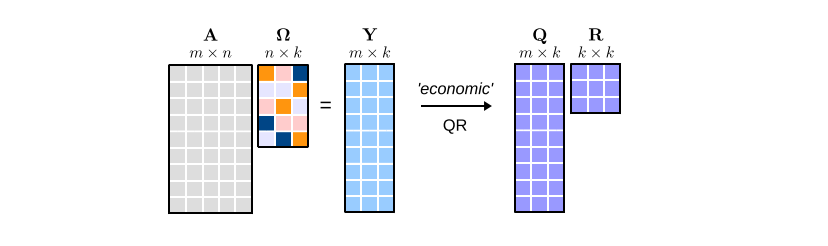
\includegraphics[width=0.8\textwidth]{assets/rsvd1.png}}
    \end{figure}
    Adapted from \cite{Erichson_2019}
\end{frame}

\begin{frame}
    \frametitle{Randomised SVD Recap}
        \begin{figure}
        \centering
        {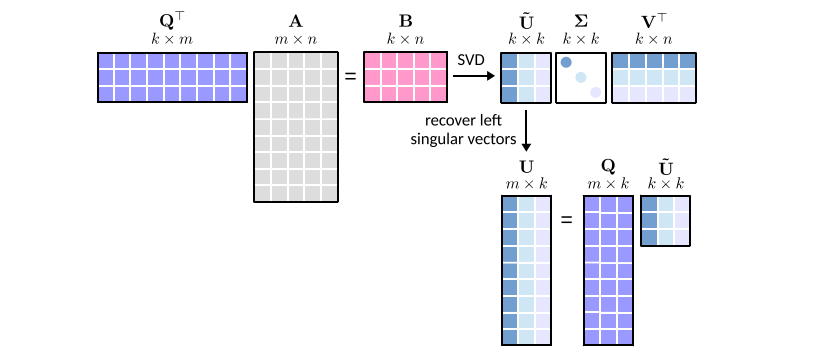
\includegraphics[width=0.8\textwidth]{assets/rsvd2.png}}
    \\Adapted from \cite{Erichson_2019}
    \end{figure}
\end{frame}

\subsection{Compressing the M2L Gram Matrix Implicitly}

\begin{frame}
    \frametitle{Compressing the M2L Gram Matrix Implicitly}
    \begin{itemize}
        \item `A' corresponds to Gram Matrix for unique M2L interactions for a given target node and up to 316 source nodes at each level
        \item We just store coordinates, and compute matrix elements implicitly, saving memory
        \item Use Cupy and Numba interoprability to transfer data to device, and compute SVD/QR algorithms - easy!
        \item Only compute unique interactions for a given level, referencing these with a `transfer vector' \cite{Fong_2009}
    \end{itemize}
\end{frame}

\subsection{Unexpected Problems}

\begin{scriptsize}
\begin{frame}
    \frametitle{Unexpected Problems}
    \begin{itemize}
        \item Need to compute a hash corresponding to a given transfer vector on the fly, can't lookup using coordinate vector as these can't be used as keys in HDF5 (or PyDict).
        \item How does one efficiently hash a vector? Does Numba support hashes? Is it fast?
        \item Inability to treat functions as first class objects (for interoprability with Cupy functions) leads to massive code duplication for different kernels.
        \item At this point, the code is already fairly UnPythonic (no objects for encapsulating behaviour, no enforced interfaces) - why are we still using Python?
    \end{itemize}
\end{frame}

\end{scriptsize}


